\protect\hyperlink{main-nav}{≡} \protect\hyperlink{close-nav}{×}

\hypertarget{section-3.8-differential-equations}{%
\section{Section 3.8: Differential
Equations}\label{section-3.8-differential-equations}}

A \textbf{differential equation} is an equation involving the derivative
of a function. They allow us to express with a simple equation the
relationship between a quantity and it's rate of change.

\hypertarget{example-1}{%
\paragraph{Example 1}\label{example-1}}

A bank pays 2\% interest on its certificate of deposit accounts, but
charges a \$20 annual fee. Write an equation for the rate of change of
the balance, \textbackslash{}( B'(t) \textbackslash{}).

If the balance \textbackslash{}( B(t) \textbackslash{}) has units of
dollars, then \textbackslash{}( B'(t) \textbackslash{}) has units of
dollars per year. When we think of what is changing the balance of the
account, there are two factors:

\begin{enumerate}
\tightlist
\item
  The interest, which increases the balance, and
\item
  The fee, which decreases the balance.
\end{enumerate}

Considering the interest, we know each year the balance will increase by
2\%, but 2\% of what? Each year that will change, since we earn interest
on whatever the current balance is. We can represent the amount of
increase as 2\% of the balance: \textbackslash{}( 0.02B(t)
\textbackslash{}) dollars/year.

The fee already has the units of dollars/year. Since everything now has
the same units, we can put the two together, and create the equation:
\textbackslash{}{[} B'(t)=0.02B(t)-20. \textbackslash{}{]}

The result is an example of a differential equation. Notice this
particular equation involves both the derivative \emph{and} the original
function, and so we can't simply find \textbackslash{}( B(t)
\textbackslash{}) using basic integration.

Algebraic equations contain constants and variables, and the solutions
of an algebraic equation are typically numbers. For example,
\textbackslash{}(x = 3\textbackslash{}) and \textbackslash{}(x =
-2\textbackslash{}) are solutions of the algebraic equation
\textbackslash{}(x\^{}2 = x + 6\textbackslash{}). Differential equations
contain derivatives or differentials of functions. Solutions of
differential equations are functions. The differential equation
\textbackslash{}(y' = 3x\^{}2\textbackslash{}) has infinitely many
solutions, and two of those solutions are the functions
\textbackslash{}(y = x\^{}3 + 2\textbackslash{}) and \textbackslash{}(y
= x\^{}3 - 4\textbackslash{}).

\begin{figure}
\centering
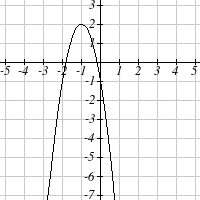
\includegraphics{images/image064.png}
\caption{}
\end{figure}

You have already solved lots of differential equations: every time you
found an antiderivative of a function
\textbackslash{}(f(x)\textbackslash{}), you solved the differential
equation \textbackslash{}(y' = f(x)\textbackslash{}) to get a solution
\textbackslash{}(y\textbackslash{}). The differential equation
\textbackslash{}(y' = f(x)\textbackslash{}), however, is just the
beginning. Other applications generate different differential equations,
like in the bank balance example above.

\hypertarget{checking-solutions-of-differential-equations}{%
\subsection{Checking Solutions of Differential
Equations}\label{checking-solutions-of-differential-equations}}

Whether a differential equation is easy or difficult to solve, it is
important to be able to check that a possible solution really satisfies
the differential equation.

A possible solution of an algebraic equation can be checked by putting
the solution into the equation to see if the result is true:
\textbackslash{}(x = 3\textbackslash{}) is a solution of
\textbackslash{}(5x + 1 = 16\textbackslash{}) since
\textbackslash{}(5(3) + 1 = 16\textbackslash{}) is true. Similarly, a
solution of a differential equation can be checked by substituting the
function and the appropriate derivatives into the equation to see if the
result is true: \textbackslash{}(y = x\^{}2\textbackslash{}) is a
solution of \textbackslash{}(xy' = 2y\textbackslash{}) since
\textbackslash{}(y' = 2x\textbackslash{}) and \textbackslash{}(x(2x) =
2\textbackslash{}left(x\^{}2\textbackslash{}right)\textbackslash{}) is
true.

\hypertarget{example-2}{%
\paragraph{Example 2}\label{example-2}}

Check (a) that \textbackslash{}(y = x\^{}2 + 5\textbackslash{}) is a
solution of \textbackslash{}(y'' + y = x\^{}2 + 7\textbackslash{}) and
(b) that \textbackslash{}(y = x +
\textbackslash{}frac\{5\}\{x\}\textbackslash{}) is a solution of
\textbackslash{}(y' + \textbackslash{}frac\{y\}\{x\} =
2\textbackslash{}).

\begin{enumerate}
\tightlist
\item
  \textbackslash{}(y = x\^{}2 + 5\textbackslash{}) so
  \textbackslash{}(y' = 2x\textbackslash{}) and \textbackslash{}(y'' =
  2\textbackslash{}). Substituting these functions for
  \textbackslash{}(y\textbackslash{}) and
  \textbackslash{}(y''\textbackslash{}) into the differential equation
  \textbackslash{}(y'' + y = x\^{}2 + 7\textbackslash{}), we have
  \textbackslash{}{[}y'' + y = (2) + \textbackslash{}left(x\^{}2 +
  5\textbackslash{}right) = x\^{}2 + 7,\textbackslash{}{]} so
  \textbackslash{}(y = x\^{}2 + 5\textbackslash{}) is a solution of the
  differential equation.
\item
  \textbackslash{}(y = x +
  \textbackslash{}frac\{5\}\{x\}\textbackslash{}) so \textbackslash{}(y'
  = 1 - \textbackslash{}frac\{5\}\{x\^{}2\}\textbackslash{}).
  Substituting these functions for \textbackslash{}(y\textbackslash{})
  and \textbackslash{}(y'\textbackslash{}) in the differential equation
  \textbackslash{}(y' + \textbackslash{}frac\{y\}\{x\} =
  2\textbackslash{}), we have \textbackslash{}{[} y' +
  \textbackslash{}frac\{y\}\{x\} = \textbackslash{}left(1 -
  \textbackslash{}frac\{5\}\{x\^{}2\}\textbackslash{}right) +
  \textbackslash{}frac\{1\}\{x\}\textbackslash{}left(x +
  \textbackslash{}frac\{5\}\{x\}\textbackslash{}right) = 1 -
  \textbackslash{}frac\{5\}\{x\^{}2\} + 1 +
  \textbackslash{}frac\{5\}\{x\^{}2\} = 2, \textbackslash{}{]} the
  result we wanted to verify.
\end{enumerate}

\hypertarget{separable-differential-equations}{%
\subsection{Separable Differential
Equations}\label{separable-differential-equations}}

A differential equation is called separable if the variables can be
separated algebraically so that all the
\textbackslash{}(x\textbackslash{})'s and
\textbackslash{}(dx\textbackslash{}) are one one side of the equation,
and all the \textbackslash{}(y\textbackslash{})'s and
\textbackslash{}(dy\textbackslash{}) are on the other side of the
equation. In other words, so the equation has the form \textbackslash{}(
f(x)\textbackslash{}, dx=g(y)\textbackslash{}, dy \textbackslash{}).

Once separated, separable differential equations can be solved by
integrating both sides of the equation.

\hypertarget{example-3}{%
\paragraph{Example 3}\label{example-3}}

Find the solution of \textbackslash{}{[}
y'=\textbackslash{}frac\{6x+1\}\{2y\}. \textbackslash{}{]}

Rewriting \textbackslash{}(y'\textbackslash{}) is a helpful first step:
\textbackslash{}{[}
\textbackslash{}frac\{dy\}\{dx\}=\textbackslash{}frac\{6x+1\}\{2y\}\textbackslash{}{]}

Now we can multiply both sides by \textbackslash{}(dx\textbackslash{})
and by \textbackslash{}(2y\textbackslash{}) to separate the variables:
\textbackslash{}{[} 2y\textbackslash{}, dy=(6x+1)\textbackslash{}, dx

Integrating each side, we have \textbackslash{}{[}
\textbackslash{}begin\{align*\} \textbackslash{}int 2y\textbackslash{},
dy=\& \textbackslash{}int (6x+1)\textbackslash{}, dx
\textbackslash{}\textbackslash{} y\^{}2+C\_1=\& 3x\^{}2+x+C\_2
\textbackslash{}end\{align*\} \textbackslash{}{]}

Notice that we can combine the two constants to create a new,
consolidated constant \textbackslash{}(C\textbackslash{}), so we usually
only bother to put a constant on the right side: \textbackslash{}{[}
y\^{}2=3x\^{}2+x+C. \textbackslash{}{]}

As expected, there is a whole family of solutions to this differential
equation.

\hypertarget{initial-value-problem-ivt}{%
\paragraph{Initial Value Problem
(IVT)}\label{initial-value-problem-ivt}}

An \textbf{initial value problem} is a differential equation that
provides additional information about the initial, or starting, value of
the function. This allows us to then solve for the constant and find a
single solution.

\hypertarget{example-4}{%
\paragraph{Example 4}\label{example-4}}

Find the solution of \textbackslash{}(
y'=\textbackslash{}frac\{6x+1\}\{2y\} \textbackslash{}) which satisfies
\textbackslash{}( y(2)=3 \textbackslash{}).

In the previous example we found the general solution, \textbackslash{}(
y\^{}2=3x\^{}2+x+C \textbackslash{}).

Substituting in the initial condition, \textbackslash{}(y =
3\textbackslash{}) when \textbackslash{}(x = 2\textbackslash{}),
\textbackslash{}{[}3\^{}2=3(2)\^{}2+2+C,\textbackslash{}{]} so
\textbackslash{}( 9=12+2+C \textbackslash{}), giving \textbackslash{}(
C=-5 \textbackslash{}).

The solution is \textbackslash{}{[} y\^{}2=3x\^{}2+x-5.
\textbackslash{}{]} Sometimes it is desirable to solve for
\textbackslash{}(y\textbackslash{}), which would yield \textbackslash{}(
y=\textbackslash{}pm\textbackslash{}sqrt\{3x\^{}2+x-5\}
\textbackslash{}), but since the initial condition had a positive
\textbackslash{}(y\textbackslash{}) value, we isolate the positive
solution: \textbackslash{}{[} y=\textbackslash{}sqrt\{3x\^{}2+x-5\}.
\textbackslash{}{]}

\hypertarget{example-5}{%
\paragraph{Example 5}\label{example-5}}

A bank pays 2\% interest on its certificate of deposit accounts, but
charges a \$20 annual fee. If you initially invest \$3,000, how much
will you have after 10 years?

You may recognize this as the example from the beginning of the section,
for which we set up the equation \textbackslash{}( B'(t)=0.02B(t)-20
\textbackslash{}) or, more simply, \textbackslash{}{[}
\textbackslash{}frac\{dB\}\{dt\}=0.02B-20. \textbackslash{}{]}

We can separate this equation by multiply by
\textbackslash{}(dt\textbackslash{}) and dividing by the entire
expression on the right: \textbackslash{}{[}
\textbackslash{}frac\{dB\}\{0.02B-20\}=dt. \textbackslash{}{]}

Integrating the left side of this equation requires substitution. Let
\textbackslash{}( u=0.02B-20 \textbackslash{}), so \textbackslash{}(
du=0.02\textbackslash{}, dB \textbackslash{}). Making the substitution,
\textbackslash{}{[} \textbackslash{}begin\{align*\}
\textbackslash{}int\textbackslash{}frac\{dB\}\{0.02B-20\}=\&
\textbackslash{}int\textbackslash{}frac\{du/0.02\}\{u\}
\textbackslash{}\textbackslash{} =\&
\textbackslash{}int\textbackslash{}frac\{1\}\{u\}\textbackslash{}frac\{du\}\{0.02\}
\textbackslash{}\textbackslash{} =\&
\textbackslash{}frac\{1\}\{0.02\}\textbackslash{}int\textbackslash{}frac\{1\}\{u\}\textbackslash{},
du \textbackslash{}\textbackslash{} =\&
\textbackslash{}frac\{1\}\{0.02\}\textbackslash{}ln\textbar{}u\textbar{}+C\_1\textbackslash{}\textbackslash{}
=\&
\textbackslash{}frac\{1\}\{0.02\}\textbackslash{}ln\textbar{}0.02B-20\textbar{}+C\_1
\textbackslash{}end\{align*\} \textbackslash{}{]}

Integrating on the right side of the differential equation is easier:
\textbackslash{}{[}\textbackslash{}int dt = t+C\_2\textbackslash{}{]}

Together, this gives us the general solution to the differential
equation (we're also combining the \textbackslash{}( C
\textbackslash{})'s in this step): \textbackslash{}{[}
\textbackslash{}frac\{1\}\{0.02\}\textbackslash{}ln\textbar{}0.02B-20\textbar{}=t+C
\textbackslash{}{]}

Now we would like to solve for \textbackslash{}(B\textbackslash{}).
Start by multiplying by 0.02. \textbackslash{}{[}
\textbackslash{}begin\{align*\}
\textbackslash{}ln\textbar{}0.02B-20\textbar{}=\& 0.02t+0.02C
\&\textbackslash{}\textbackslash{}
\textbackslash{}ln\textbar{}0.02B-20\textbar{}=\& 0.02t+D
\&\textbackslash{}qquad\textbackslash{}text\{We can rename
\textbackslash{}( D=0.02C \textbackslash{}) for
simplicity.\}\textbackslash{}\textbackslash{}
e\^{}\{\textbackslash{}ln\textbar{}0.02B-20\textbar{}\}=\&
e\^{}\{0.02t+D\}
\&\textbackslash{}qquad\textbackslash{}text\{Exponentiate both sides:
\textbackslash{}(
e\^{}\{\textbackslash{}text\{left\}\}=e\^{}\{\textbackslash{}text\{right\}\}
\textbackslash{}).\}\textbackslash{}\textbackslash{}
\textbar{}0.02B-20\textbar{}=\& e\^{}\{0.02t+D\}
\&\textbackslash{}qquad\textbackslash{}text\{Use the log rule
\textbackslash{}( e\^{}\{\textbackslash{}ln(A)\}=A
\textbackslash{}).\}\textbackslash{}\textbackslash{} 0.02B-20=\&
e\^{}\{0.02t+D\} \&\textbackslash{}qquad\textbackslash{}text\{Since the
RHS is always positive, we can drop the abs
value.\}\textbackslash{}\textbackslash{} 0.02B-20=\&
e\^{}\{0.02t\}e\^{}D \&\textbackslash{}qquad\textbackslash{}text\{Using
the rule \textbackslash{}( e\^{}\{A+B\}=e\^{}Ae\^{}B
\textbackslash{}).\}\textbackslash{}\textbackslash{} 0.02B-20=\&
ke\^{}\{0.02t\} \&\textbackslash{}qquad\textbackslash{}text\{Rename
\textbackslash{}( k=e\^{}D
\textbackslash{}).\}\textbackslash{}\textbackslash{} B=\&
\textbackslash{}frac\{ke\^{}\{0.02t\}+20\}\{0.02\}=\textbackslash{}frac\{ke\^{}\{0.02t\}\}\{0.02\}+1000
\&\textbackslash{}qquad\textbackslash{}text\{Add 20 and divide by
0.02.\}\textbackslash{}\textbackslash{} B=\& Ae\^{}\{0.02t\}+1000
\&\textbackslash{}qquad\textbackslash{}text\{Rename \textbackslash{}(
A=\textbackslash{}frac\{k\}\{0.02\} \textbackslash{}).\}
\textbackslash{}end\{align*\} \textbackslash{}{]}

Finally, we can substitute our initial value of \textbackslash{}(B =
3000\textbackslash{}) when \textbackslash{}(t = 0\textbackslash{}) to
solve for the constant \textbackslash{}(A\textbackslash{}):
\textbackslash{}{[} \textbackslash{}begin\{align*\} 3000=\&
Ae\^{}\{0.02(0)\}+1000 \textbackslash{}\textbackslash{} A=\& 2000
\textbackslash{}end\{align*\} \textbackslash{}{]}

This gives us the equation for the account balance after
\textbackslash{}(t\textbackslash{}) years: \textbackslash{}{[}
B(t)=2000e\^{}\{0.02t\}+1000. \textbackslash{}{]}

To find the balance after 10 years, we can evaluate this equation at
\textbackslash{}(t = 10\textbackslash{}): \textbackslash{}{[}
B(10)=2000e\^{}\{0.02(10)\}+1000\textbackslash{}approx
\textbackslash{}\$3442.81. \textbackslash{}{]}

It's worth noting that this answer isn't exactly right. Differential
equations assume \emph{continuous} changes, and it is unlikely interest
is compounded continuously or the fee is extracted continuously.
However, the answer is probably close to the actual answer, and
differential equations provide a relatively simple model of a
complicated situation.

\hypertarget{models-of-growth}{%
\subsection{Models of Growth}\label{models-of-growth}}

The bank account example demonstrated one basic model of growth: growth
proportional to the existing quantity. Bank accounts and populations
both tend to grow this way if not constrained. This type of growth is
called \textbf{unlimited growth}.

\hypertarget{unlimited-growth}{%
\paragraph{Unlimited Growth}\label{unlimited-growth}}

If a quantity or population y grows at a rate proportional that
quantity's size, it can be modeled with unlimited growth, which has the
differential equation: \textbackslash{}{[} y'=ry, \textbackslash{}{]}
where \textbackslash{}(r\textbackslash{}) is a constant.

\hypertarget{example-6}{%
\paragraph{Example 6}\label{example-6}}

A population grows by 8\% each year. If the current population is 5,000,
find an equation for the population after
\textbackslash{}(t\textbackslash{}) years.

\textbackslash{}{[} \textbackslash{}begin\{align*\}
\textbackslash{}frac\{dy\}\{dt\}=\& 0.08y
\&\textbackslash{}\textbackslash{}
\textbackslash{}frac\{1\}\{y\}\textbackslash{}, dy=\&
0.08\textbackslash{}, dt
\&\textbackslash{}qquad\textbackslash{}text\{Separate the
variables.\}\textbackslash{}\textbackslash{}
\textbackslash{}ln\textbar{}y\textbar{}=\& 0.08t+C
\&\textbackslash{}qquad\textbackslash{}text\{Integrate both
sides.\}\textbackslash{}\textbackslash{}
e\^{}\{\textbackslash{}ln\textbar{}y\textbar{}\}=\& e\^{}\{0.08t+C\}
\&\textbackslash{}qquad\textbackslash{}text\{Exponentiate both
sides.\}\textbackslash{}\textbackslash{} y=\& Ae\^{}\{0.08t\}
\&\textbackslash{}qquad\textbackslash{}text\{Simplify both sides, using
the tricks we used in the bank example.\} \textbackslash{}end\{align*\}
\textbackslash{}{]}

Now substitute in the initial condition: \textbackslash{}(
5000=Ae\^{}\{0.08(0)\} \textbackslash{}), so \textbackslash{}( A=5000
\textbackslash{}).

The population will grow following the equation \textbackslash{}{[}
y=5000e\^{}\{0.08t\}. \textbackslash{}{]}

Notice that the solution to the unlimited growth equation is an
exponential equation.

When a product is advertised heavily, sales will tend to grow very
quickly, but eventually the market will reach saturation, and sales will
slow. In this type of growth, called \textbf{limited growth}, the
population grows at a rate proportional to the distance from the maximum
value.

\hypertarget{limited-growth}{%
\paragraph{Limited Growth}\label{limited-growth}}

If a quantity grows at a rate proportional to the distance from the
maximum value, \textbackslash{}(M\textbackslash{}), it can be modeled
with limited growth, which has the differential equation
\textbackslash{}{[} y'=k(M-y), \textbackslash{}{]} where
\textbackslash{}(k\textbackslash{}) is a constant, and
\textbackslash{}(M\textbackslash{}) is the maximum size of
\textbackslash{}(y\textbackslash{}).

\hypertarget{example-7}{%
\paragraph{Example 7}\label{example-7}}

A new cell phone is introduced. The company estimates they will sell 200
thousand phones. After 1 month they have sold 20 thousand. How many will
they have sold after 9 months?

In this case there is a maximum amount of phones they expect to sell, so
\textbackslash{}(M = 200\textbackslash{}) thousand. Modeling the sales,
\textbackslash{}(y\textbackslash{}), in thousands of phones, we can
write the differential equation \textbackslash{}{[} y'=k(200-y).
\textbackslash{}{]}

Since it was a new phone, \textbackslash{}( y(0)=0 \textbackslash{}). We
also know the sales after one month, \textbackslash{}( y(1)=20
\textbackslash{}).

Solving the differential equation: \textbackslash{}{[}
\textbackslash{}begin\{align*\} \textbackslash{}frac\{dy\}\{dt\}=\&
k(200-y) \&\textbackslash{}\textbackslash{}
\textbackslash{}frac\{dy\}\{200-y\}=\& k\textbackslash{}, dt
\&\textbackslash{}qquad\textbackslash{}text\{Separate the
variables.\}\textbackslash{}\textbackslash{}
-\textbackslash{}ln\textbar{}200-y\textbar{}=\& kt+C
\&\textbackslash{}qquad\textbackslash{}text\{Integrate both sides. On
the left use the substitution.\}\textbackslash{}\textbackslash{}
e\^{}\{\textbackslash{}ln\textbar{}200-y\textbar{}\}=\& e\^{}\{-kt+C\}
\&\textbackslash{}qquad\textbackslash{}text\{Multiply both sides by -1,
and exponentiate both sides.\}\textbackslash{}\textbackslash{} 200-y=\&
Be\^{}\{-kt\}
\&\textbackslash{}qquad\textbackslash{}text\{Simplify.\}\textbackslash{}\textbackslash{}
y=\& Ae\^{}\{-kt\}+200
\&\textbackslash{}qquad\textbackslash{}text\{Subtract 200, divide by -1,
and simplify.\} \textbackslash{}end\{align*\} \textbackslash{}{]}

Using the initial condition \textbackslash{}( y(0)=0 \textbackslash{}),
\textbackslash{}{[} 0=Ae\^{}\{-k(0)\}+200, \textbackslash{}{]} so
\textbackslash{}( 0=A+200 \textbackslash{}), giving \textbackslash{}(
A=-200 \textbackslash{}).

Using the value \textbackslash{}( y(1)=20 \textbackslash{}):
\textbackslash{}{[} \textbackslash{}begin\{align*\} 20=\&
-200e\^{}\{-k(t)\}+200 \&\textbackslash{}\textbackslash{}
\textbackslash{}frac\{=180\}\{-200\}=\& 0.9=e\^{}\{-k\}
\&\textbackslash{}qquad\textbackslash{}text\{Subtract 200 and divide
-200.\}\textbackslash{}\textbackslash{} \textbackslash{}ln(0.9)=\&
\textbackslash{}ln\textbackslash{}left(e\^{}\{-k\}\textbackslash{}right)=-k
\&\textbackslash{}qquad\textbackslash{}text\{Take the ln of both
sides.\}\textbackslash{}\textbackslash{} k=\&
-\textbackslash{}ln(0.9)\textbackslash{}approx 0.105
\&\textbackslash{}qquad\textbackslash{}text\{Divide by -1.\}
\textbackslash{}end\{align*\} \textbackslash{}{]}

As a quick sanity check, this value is positive as we would expect,
indicating that the sales are growing over time. We now have the
equation for the sales of phones over time: \textbackslash{}{[}
A=-200e\^{}\{-0.105t\}+200. \textbackslash{}{]}

Finally, we can evaluate this at \textbackslash{}(t = 9\textbackslash{})
to find the sales after 9 months: \textbackslash{}{[}
A(9)=-200e\^{}\{-0.105(9)\}+200\textbackslash{}approx
122.26\textbackslash{}text\{ thousand phones\}. \textbackslash{}{]}

Limited growth is also commonly used for learning models, since when
learning a new skill, people typically learn quickly at first, then
their rate of improvement slows down as they approach mastery.

Earlier we used unlimited growth to model a population, but often a
population will be constrained by food, space, and other resources. When
a population grows both proportional to its size, and relative to the
distance from some maximum, that is called \textbf{logistic growth}.
This leads to the differential equation \textbackslash{}( y'=ky(M-y)
\textbackslash{}), which is accurate but not always convenient to use.
We will use a slight modification. Since solving this differential
equation requires integration techniques we haven't learned, the
solution form is given.

\hypertarget{logistic-growth}{%
\paragraph{Logistic Growth}\label{logistic-growth}}

If a quantity grows at a rate proportional to its size and to the
distance from the maximum value, \textbackslash{}(M\textbackslash{}), it
can be modeled with \textbf{logistic growth}, which has the differential
equation: \textbackslash{}{[}
y'=ry\textbackslash{}left(1-\textbackslash{}frac\{y\}\{M\}\textbackslash{}right).
\textbackslash{}{]}

\textbackslash{}(r\textbackslash{}) can be interpreted as ``the growth
rate absent constraints'', i.e., how the population would grow if there
wasn't a maximum value.

This differential equation has solutions of the form \textbackslash{}{[}
y=\textbackslash{}frac\{M\}\{1+Ae\^{}\{-rt\}\}. \textbackslash{}{]}

\hypertarget{example-8}{%
\paragraph{Example 8}\label{example-8}}

A colony of 100 rabbits is introduced to a reclaimed forest. After 1
year, the population has grown to 300. It is estimated the forest can
sustain 5000 rabbits. The forest service plans to reintroduce wolves to
the forest when the rabbit population reaches 3000 rabbits. When will
that occur?

The maximum sustainable population was given as \textbackslash{}(M =
5000\textbackslash{}). Using the solution form \textbackslash{}{[}
y=\textbackslash{}frac\{M\}\{1+Ae\^{}\{-rt\}\} \textbackslash{}{]} and
the initial condition \textbackslash{}( y(0)=100 \textbackslash{}) we
can solve for \textbackslash{}( A \textbackslash{}): \textbackslash{}{[}
\textbackslash{}begin\{align*\} 100=\&
\textbackslash{}frac\{5000\}\{1+Ae\^{}\{-r(0)\}\}
\&\textbackslash{}\textbackslash{} 100=\&
\textbackslash{}frac\{5000\}\{1+A\}
\&\textbackslash{}qquad\textbackslash{}text\{Simplify.\}\textbackslash{}\textbackslash{}
100(1+A)=\& 5000 \&\textbackslash{}qquad\textbackslash{}text\{Multiply
both sides by \textbackslash{}( 1+A
\textbackslash{}).\}\textbackslash{}\textbackslash{} 1+A=\& 50
\&\textbackslash{}qquad\textbackslash{}text\{Divide by
100.\}\textbackslash{}\textbackslash{} A=\& 49 \&
\textbackslash{}end\{align*\} \textbackslash{}{]}

Now, using \textbackslash{}( y(1)=300 \textbackslash{}), we can solve
for \textbackslash{}(r\textbackslash{}): \textbackslash{}{[}
\textbackslash{}begin\{align*\} 300=\&
\textbackslash{}frac\{5000\}\{1+49e\^{}\{-r(1)\}\}
\textbackslash{}\textbackslash{}
300\textbackslash{}left(1+49e\^{}\{-r\}\textbackslash{}right)=\& 5000
\textbackslash{}\textbackslash{} 1+49e\^{}\{-r\}=\&
\textbackslash{}frac\{5000\}\{300\} \textbackslash{}\textbackslash{}
e\^{}\{-r\}=\&
\textbackslash{}frac\{\textbackslash{}frac\{50\}\{3\}-1\}\{49\}\textbackslash{}approx
0.3197 \textbackslash{}\textbackslash{} -r=\& \textbackslash{}ln(0.3197)
\textbackslash{}\textbackslash{} r=\&
-\textbackslash{}ln(0.3197)\textbackslash{}approx 1.1404
\textbackslash{}end\{align*\} \textbackslash{}{]}

We now have the equation for the population after
\textbackslash{}(t\textbackslash{}) years: \textbackslash{}{[}
y=\textbackslash{}frac\{5000\}\{1+49e\^{}\{-1.1404t\}\}.
\textbackslash{}{]}

To answer the original equation, of when the rabbit population will
reach 3000, we need to solve for \textbackslash{}(t\textbackslash{})
when \textbackslash{}(y = 3000\textbackslash{}): \textbackslash{}{[}
\textbackslash{}begin\{align*\} 3000=\&
\textbackslash{}frac\{5000\}\{1+49e\^{}\{-1.1404t\}\}
\textbackslash{}\textbackslash{}
3000\textbackslash{}left(1+49e\^{}\{-1.1404t\}\textbackslash{}right)=\&
5000 \textbackslash{}\textbackslash{} e\^{}\{-1.1404t\}=\&
\textbackslash{}frac\{\textbackslash{}frac\{5\}\{3\}-1\}\{49\}\textbackslash{}approx
0.01361 \textbackslash{}\textbackslash{} t=\&
\textbackslash{}frac\{\textbackslash{}ln(0.01361)\}\{-1.1404\}\textbackslash{}approx
3.77\textbackslash{}text\{ years\}. \textbackslash{}end\{align*\}
\textbackslash{}{]}

Logistic growth is also a good model for unadvertised sales. A new
product that is not advertised will have sales increase slowly at first,
then grow as word of mouth spreads and people become familiar with the
product. Sales will level off as they approach market saturation.

\begin{longtable}[]{@{}ll@{}}
\toprule
\endhead
\href{section3-7.php}{← Previous Section} &
\href{../chapter4/section4-1.php}{Next Section →}\tabularnewline
\bottomrule
\end{longtable}
